\documentclass[12pt,twocolumn]{article}
\usepackage{graphicx}
\usepackage{pdfpages}
\usepackage{hyperref}
\usepackage[margin=1.25in]{geometry}
\usepackage[utf8]{inputenc}
\graphicspath{ {./Figures/} }
\hypersetup{
    colorlinks=true,
    linkcolor=blue,
    filecolor=magenta,      
    urlcolor=cyan,
}
\urlstyle{same}
\usepackage[font={small,it}]{caption}
\usepackage{fancyvrb}
\title{Model \& Simulation of South Bend Government Call Center using Arena}
\author{John D. Bulger, Jacob D. White \& Adali J.J. Johnson\\Valparaiso University\thanks{``We have neither given or received, nor have we tolerated others' use of unauthorized aid."}}
\date{October 25, 2018}

	\begin{document}
\maketitle

\section{Introduction}
The city of South Bend, located in northern Indiana, established a citizen-accessible call center in February 2013.  It addresses almost every aspect of city-citizen interaction, including waste pick-up and removal, water billing and disconnections, and code enforcement.  By serving as a central hub for communication, the call center is able to consolidate a substantial amount of data regarding citizens as consumers.  This data is available on South Bend's open data portal at \textit{https://data-southbend.opendata.arcgis.com}.

	\begin{figure}[h]
	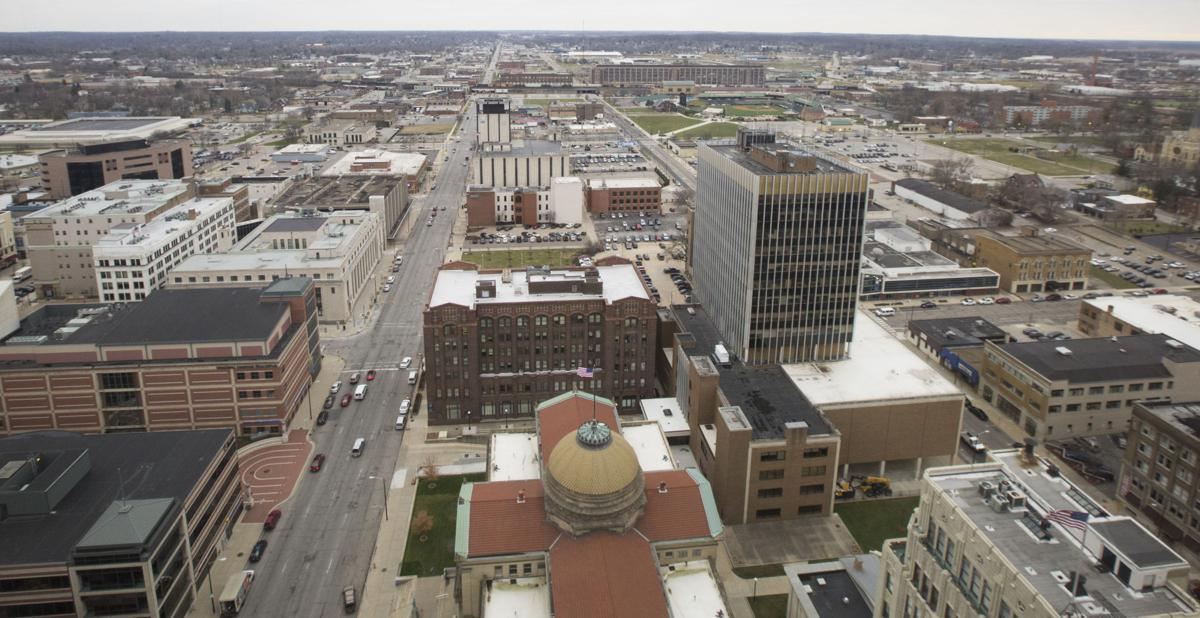
\includegraphics[scale=.17]{south_bend.png}
	\caption{South Bend, IN (Greg Swiercz)}
	\end{figure}

\par
The city's call center is seeking to explore operational efficiency with regard to operator staff.  As such, this model and simulation will be constructed with the primary purpose of discovering the optimal number of agents while maintaining adequate customer satisfaction (measured by time in queue).  Additionally, the model will be modified to explore the addition of a self-service touch-tone option that would allow for callers to complete simple tasks, such as scheduling an extra trash pickup, without speaking to an agent.  Through simulation, these questions will be explored and potential solutions will be posited.  The open-source data was processed in Python in order to extract relevant distributions, and the call center was modeled in Arena as a discrete-event model.  

\section{Background}
Call centers are a frequently studied topic within the simulation and modeling disciplines.  As such, some basic terminology shall be explained.  This model consists of two primary components:  calls and operators.  Calls will be represented as entities in Arena.  As entities, they can be created on distributions found from the data processing and then can properly flow through the simulation to a disposal point.  For this exploration, an ``arrival" is defined as a unique call first coming into the call process model.  The operators, also known as ``311 liasons," will be represented as resources in Arena.  As resources, the operators can be seized by the incoming call entities to properly simulate their time spent on each call.

	\subsection{Prior Work}

As stated previously, call centers are a frequently studied topic within simulation and modeling disciplines.  As such, call centers are a prime opportunity to utilize simulation techniques.  In fact, according to Bapat and Pruitte, simulation is the preferred method to analyze and determine the effectiveness of a call center.\cite{bapat}  It allows for evaluation of metrics beyond what a basic analysis encompasses.  For example, the scheduling of call agents should be optimized against call duration and abandonment, as documented by Saltzman and Mehrota\cite{saltzman}.  Such simulations can easily be created to illustrate feasibility of goal accomplishment for corporations while enabling efficient and accurate decision-making\cite{saltzmeh}.

\par


Call center and queuing analysis has been the focus of academic research for years.  Brown et al. provide an excellent overview of the Poisson distribution modeling customer arrivals, as well as the accompanying assumptions\cite{brown}.  While arrival distribution is analyzed directly from the data in this model, it will still be implemented as an hourly Poisson distribution. In order to implement this arrival methodology, the authors maintain assumptions that the customers and operators are statistically identical and that they all act independently.  Zhang, Hong, and Zhang also describe the arrival process as a Poisson distribution, but discuss models which may be more accurate alternatives\cite{zhang}.  They maintain some of the main assumptions as Brown et al.  Additionally, they point out that differences in time-dependent parameters, customer attitudes and preferences, and operator skill levels should be treated as negligible when it comes to their impact on the simulation results.


\section{Mathematical Model}

Our core model structure is based off the work of Mandelbaun in 2001\cite{mandelbaun}.  In his highly esteemed text, Mandelbaun lays out the basic schematic of a call center model.  His model illustrates the possible flow of a call, starting with its arrival until disposal, be that as a lost call or having completed successfully.  While simplistic by nature, the model covers all of the basic aspects of a call center in a sensible format that can easily by applied in Arena.  This model can be seen in Figure 2.  

	\begin{figure}[h]
	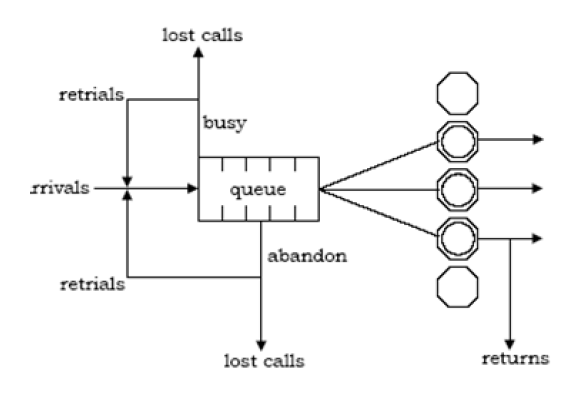
\includegraphics[scale=.45]{call_center_layout.png}
	\caption{Basic Operational Schematic of Call Center (Mandelbaun 2001)}
	\end{figure}

Mandelbaun's model identifies one avenue for arrivals (incoming calls) and three methods of disposal(lost calls due to busy signal, lost calls due to wait time, and completed calls).  It can be seen that the lost calls due to busy signals and the lost calls due to wait time both have retrial loops built in where some customers may immediately try to call into the system again and are treated as new arrivals for the sake of the simulation.  Additionally, completed calls have the option to ``return", where they would immediately re-enter the system for whatever reason (perhaps an unresolved issue).  There is a single centralized queue before the calls are distributed among resources (operators).  At its core, this is a condensed high-level view of a call center model, specifically designed so that it could easily be expanded as needed for specific analysis.

\subsection{Expanded Model}
The model used for this analysis expands a great deal on the core model identified by Mandelbaun.  It adds three key features that the original model omits: voicemails, operator breaks, and alternate call flow for supervisor assistance.  Additionally, calls are assigned key attributes that determine their specific flow and timing throughout the simulation.  These key attributes include topic, language, and priority.

	\paragraph{Voicemails}
	
In addition to arriving calls, voicemails are ``created" as soon as each simulation ``day" begins, so that the call center has all day to return those calls.  These are considered a lower priority item for the call center operators.  A constant number of voicemails are received by the call center immediately at the beginning of each simulated day to represent the voicemails that built up the night before.

	\paragraph{Operator Breaks}
	
To try and obtain more accurate results, the operator resources were given ``breaks" to better simulate potential slow downs due to operator time off. Break scheduling is different for full-time and part-time employees, so both were taken into account for the simulation.

	\paragraph{Supervisor}
	
Some calls get routed to a supervisor after speaking with an agent.  This supervisor resource can then resolve the call, or pass it back to an agent.  This was added in an attempt to model actual call center behavior, where some callers may need assistance beyond a basic operator or may request supervisor assistance for a dispute. 

	\paragraph{Topic}

Calls are assigned a topic based on the distribution of topics in historical call center data.  In an effort to preserve the simplicity of the model while still utilizing past data, the top six departments (by total number of calls) are specified, with the remaining calls grouped into an ``other" category.  By assigning a topic, the simulation will be able to utilize the historical mean and standard deviation of those topics' call durations in order to more accurately replicate the call center.  The departments specifically included in the model account for 90\% of the total call volume in the original source data, while the ``other" category constitutes the remaining 10\%.  This is illustrated in Figure 3.

	\paragraph{Self-Service}
	
One of the purposes of this project is to evaluate the impact of adding a self-service option that would eliminate the need to speak to an agent for certain call topics.  This was added as an extension of the base model, but was run separately from the base model for the use of direct comparison of the results.  Depending on the assigned call topic, callers have the option to self-service, with multiple routes leading to the agent queue in the event the caller has trouble with self-service and needs an operator.


\begin{figure}[h]
	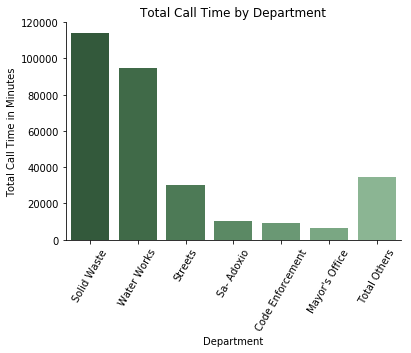
\includegraphics[scale=.53]{Calls_Department_sim.png}
	\caption{Call distribution by department from source data}
\end{figure}

	\paragraph{Language}

Each call and voicemail is assigned a language of either Spanish or English.  The actual call center deals in both of those language, and it has Spanish-speaking operators available.  In order to reflect this, the model's resources all speak English, with some able to speak Spanish as well.  Therefore, arrivals will be routed into two queues:  one for English, and one for Spanish.  Historical data regarding this distribution was not immediately available, so this is modeled as an estimated parameter that was generated from the population demographics of South Bend.

	\paragraph{Priority}

All incoming calls are assigned a medium priority by default and all voicemails are given a low priority by default (as they can be answered and returned as time permits).  After speaking to an agent, calls needing escalation to a supervisor are given the highest priority (in the event they need to cycle back through the queue again).


\section{Verification \& Validation}

	\subsection{Verification Techniques}

The model and simulation was verified using two primary techniques.  First, the model was tested and run in stages, using simplified or constant parameters.  For example, voicemails were not created and queues were eliminated in order to most simply ensure the call arrival and attribute assignment worked as expected.  A similar process was repeated with voicemails and excluding call arrivals.  Resources (operators and supervisor) were reduced to one at a time and stepped through in order to ensure proper call processing treatment.  

\par

The model was also verified by ensuring the output matched the estimated results produced from a static analysis.  As an example, this includes the comparison of the total number of calls, number of dropped calls, and number of operator breaks for a given simulation period.  An average week of simulation yielded a total of 2,586 calls, with static analysis suggesting an average of 2,505.  The simulation also yielded the correct number of breaks given the number of full-time and part-time employees that worked on a given replication.  The static analysis was computed by taking the sum of arrivals from the arrival schedule (a Poisson distribution) with no regard for randomness.  These values affirm the results being generated from the simulation.
	
	
	\subsection{Validation Plan}
	
The model and simulation's results were ultimately validated using historical data.  Since we possess several years' worth of call center data, the results of the base simulation can be compared to this historical data.  As an example, the replication mentioned earlier yielded 2,586 weekly incoming calls.  Historical data suggests a total of 2,650 calls per week.  Again, these numbers can be seen as affirmation for the purposes of this simulation.  Call duration (determined by topic) was also created from the historical data, so this is easily validated as well.  The operator schedule was provided by call center management, ensuring historical validation for these values.  Historical data also exists for percent of calls abandoned, which can also be directly compared.
	
\section{Simulation}

	\subsection{Techniques and Language}
	
A call center is modeled as a discrete event model, leading to the logical choice of Arena for this simulation.  Arena excels in creating and monitoring entities, while providing a visual representation of their flow through a system (calls through a call center in this case).  Arena allows for efficient statistic and metric collection, which can be organized and analyzed to answer any questions initially posed for the simulation.

\par

Arena also features built-in modules that vastly simplify actions that would need to intricately programmed in a high-level language.  A prime example of this could be Arena's ``schedule" option.  A Poisson distribution, broken down by hourly duration, is a built-in option that was leveraged for two aspects of this project:  the call arrival schedule and call center operator schedule.  By using this included module, the simulation was able to be developed as close to ``real-life" as possible in these areas.
	
	\subsection{Attributes \& Resources}

Three main attributes are assigned to entities upon entry to the system:  topic, language, and priority.  Topic serves as a determinant of the call duration distribution, and is pulled from historical data.  Language is assigned to be either English or Spanish, and the distribution is based on the South Bend Hispanic population percentage.  While other residents surely speak other native languages, the call center only deals internally with English or Spanish, and this simulation is set up to reflect this.  Priority is assigned as a ``medium" for incoming calls, ``low" for voicemails to be returned, and ``high" for calls routed to or from a supervisor.

\par

Two resources exist in this call center model:  call center liaisons (operators) and supervisors.  The operator schedule (and thus total resources at any given simulation time) was based on the historical data as opposed to being an estimated parameter.  This schedule can be seen in Figure 4.  In keeping with typical call center model processes as described by Zhang, these operators are treated as having the same skill level, and thus do not influence the handling of a call \cite{zhang}.  Supervisors handle calls identified as problematic, but are again treated as if they are of the same skill level.  Operator lunches and personal breaks are also based on the schedule provided.

	\begin{figure}[h]
		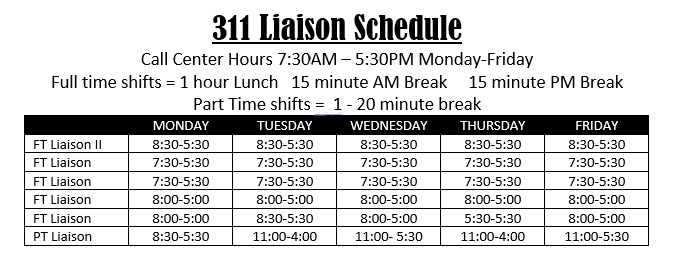
\includegraphics[scale=.3]{schedule2.jpg}
		\caption{Call center operator schedule}
	\end{figure}
	
	\subsection{Parameters}
	
	
	This simulation utilizes an accurate representation of arrivals as calculated from the aforementioned open-source data.  Mean call arrivals were identified down to the hour for each weekday.  This allows for the simulation to not only pick up on historical call patterns by hour, but also the differences between each day.  The results allow for the arrivals to be scheduled as such in Arena.  This will base the actual volume of calls in line with prior historical trends, as opposed to applying a rough blanket estimate.
	
	\par
	
	Several other estimated parameters exist in this model and simulation.  These included callers getting a busy signal (and the corresponding retry rate), callers who experience a problem and need to speak with a supervisor, and whether calls who spoke to a supervisor need to be transferred back to an agent to complete a task.  These parameters were estimated through the use of research and experimentation in an effort to represent the center as closely as possible, since no data existed for these.
	
	\subsection{Run Settings \& Replications}
	
	 The call center is open five days a week, from 7:30 AM to 5:30 PM.  Therefore, the simulation was run for 26 replications of five ten-hour days.  This works out to a half-year period (not accounting for holidays or other days where the call center may be closed).  This span of time was decided upon to try and allow for enough replications for the call center arrival distributions to approach the actual call data's distribution.
	 
	 
	\subsection{Adjustments for Self-Serve Option Model}
	
	The base model was expanded upon into a second model in order to evaluate the effectiveness of adding a self-service alternative before speaking to an agent.  The ``route" for calls to self-service utilized empirical research regarding consumer attitudes for automated systems.  A survey by Nuance Enterprise suggests that up to 75\% of consumers see self-service as a convenient option when available while 67\% said they preferred self-service over dealing with a company representative \cite{webblog}.  The simulation utilizes the 67\% preference to determine the number of call arrivals that will be routed into self-service options, given the customer has been assigned a topic that is self-serviceable.  All remaining calls were routed to the operator queue discussed in the original model.

\section{Results}

	\subsection{Number of Operators}
	
	
	\subsection{Self-Service Call Option}

\section{Discussion}



\section{Conclusion}

	\subsection{Challenges}

	\subsection{Opportunities for Further Study}














\newpage
\clearpage
\pagenumbering{gobble}
\begin{thebibliography}{8}
	
	\bibitem{bapat}
	Bapat, V. \& Pruitte, E.B. Jr.. (1998). Using simulation in call centers. \textit{In Proceedings of the 30th conference on Winter simulation (WSC '98)}, D. J. Medeiros, Edward F. Watson, John S. Carson, and Mani S. Manivannan (Eds.). IEEE Computer Society Press, Los Alamitos, CA, USA, 1395-1400.
	
	\bibitem{saltzman}
	Saltzman, R.M. \& Mehrotra, V.. (2007). Managing trade-offs in call center agent scheduling: methodology and case study. \textit{In Proceedings of the 2007 Summer Computer Simulation Conference (SCSC '07)}. Society for Computer Simulation International, San Diego, CA, USA, 643-651.
	
	\bibitem{saltzmeh}
	Saltzman, R.M. \& Mehrota, V. (2001). A call center uses simulation to drive strategic change. \textit{Interfaces 31}(3). https://doi.org/10.1287/inte.31.3.87.9632.
	
	
	\bibitem{baraka}
	Baraka, H., Baraka H. \& El-Gamily, I. (2013). Assessing call centers' success: A validation of the DeLone and Mclean model for information system. \textit{Egyptian Informatics Journal, 14}, 99-108.

	\bibitem{brown}
	Brown, L., Gans, N., Mandelbaum, A., Sakov, A., Shen, H., Zeltyn, S., \& Zhao, L. (2005). Statistical analysis of a telephone call center: a queueing-science perspective. \textit{Journal of the American Statistical Association, 100}(469), 36-50.

	\bibitem{zhang}
	Zhang X., Jeff Hong L., \& Zhang J.. (2014). Scaling and modeling of call center arrivals. \textit{In Proceedings of the 2014 Winter Simulation Conference (WSC '14)}. IEEE Press, Piscataway, NJ, USA, 476-485.

	\bibitem{mandelbaun}
	Mandelbaun A., Sakov A., \& Zeltyn S.. (2001). Empirical Analysis of a Call Center. Technion Israel Institute of Technology, Israel.
	
	\bibitem{webblog}
	Finlay, A. (2018, August 10) \textit{It’s Not You, It’s Bots: Why Some Customers Prefer Self-Service Support Over Human Support Agents}. Retrieved from https://thinkrelay.com/blog/self-service-support/.

\end{thebibliography}

\end{document}